\chapter{Metódy výpočetnej predikcie}
Cieľom výpočetnej predikcie RNA štruktúry je dokázať algoritmicky modelovať terciárnu alebo sekundárnu štruktúru na základe znalosti primárnej sekvencie RNA molekuly. Pri takejto predikcii je dôležité, aby sme dostali čo najpresnejší výsledok v porovnaní s experimentálnymi metódami, a zároveň aby výpočtové nároky a čas boli výrazne nižšie, než v prípade experimentálnej rezolúcie štruktúry. Aby malo zmysel sa pokúšať o predikciu štruktúry zo sekvencie potrebujeme vedieť, že terciárna a teda aj sekundárna štruktúra je do veľkej miery jednoznačne určená štruktúrou primárnou.  


\indent Túto otázku môžeme zodpovedať vďaka znalostiam zo skladania (foldingu) proteínov, ktorých výskumu sa venovalo viacej úsilia. Platí, že skladanie bielkovín a RNA prebieha veľmi podobne, a preto poznatky o štruktúrach a sekvenciách bielkovín môžeme použiť aj pri RNA. \cite{Moore99} 


\indent  Existujú dve hlavné pozorovania, ktoré nám umožnujú štruktúry makromolekúl modelovať  \cite{Jenny09}:
\begin{itemize}
\item Štruktúra proteínu je unikátne určená sekvenciou aminokyselín.
\item Štruktúra sa zachováva aj pri určitých zmenách v sekvencii, a teda platí, že napriek odlišnosti v sekvenciách sú štruktúry veľmi podobné. Je to spôsobené tým, že počas evolúcie štruktúra stále plnila podobnú úlohu, a preto sa jej tvar nemenil aj napriek mutáciám sekvencie. Vďaka rozširujúcej sa databáze makromolekúl (Protein Data Bank) boli získané vzťahy určujúce, aká musí byť podobnosť rovnako dlhých sekvencií, aby sme mohli predpokladať, že aj ich štruktúry sú podobné. Tento vzťah zobrazuje obrázok  \ref{obr01:aln-zones}.
\end{itemize}

\begin{figure}%[p]\centering
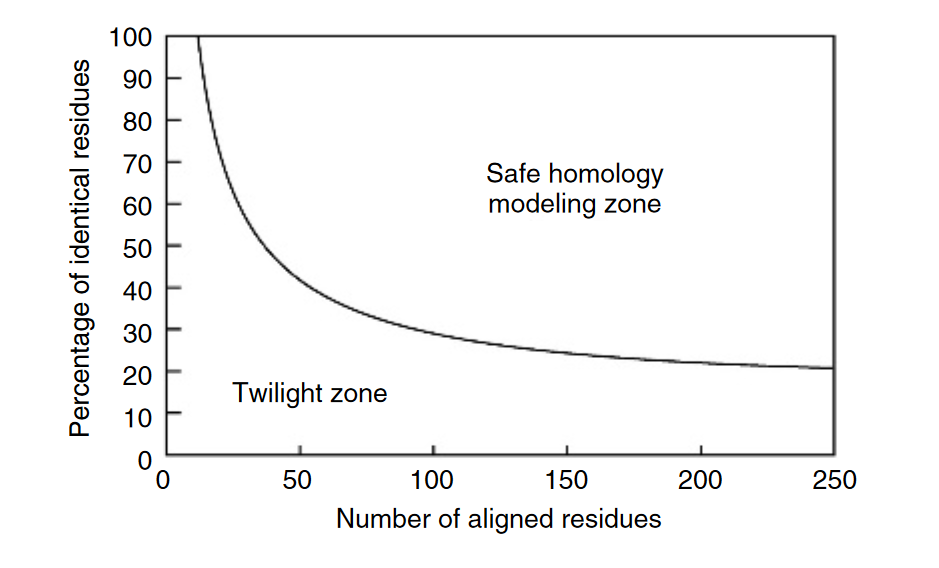
\includegraphics[width=\textwidth]{../img/zones_of_aln}
\caption{Vzťah dĺžky štruktúr a percentuálneho pomeru identických residuí v sekvenciách určujúce predpoklad, že štruktúry takýchto sekvencií sú podobné. \cite{Jenny09}}
\label{obr01:aln-zones}
\end{figure}

\section{Ab initio predikcia}
Pri ab initio predikcii štruktúry vychádzame iba z primárnej sekvencie a chemicko-fyzikálnych vlastností, vďaka ktorým sa v reálnom svete štruktúra skladá do stabilného tvaru. Algoritmus postupne vytvára kandidátske štruktúry tak, že sa snaží minimalizovať funkciu predstavujúcu voľnú energiu (energia, ktorá je ľahko dostupná v systéme). Následne z takto vygenerovaných kandidátov musí vybrať najprirodzenejšiu štruktúru. Najväčším problémom tohoto prístupu je mnoho lokálnych miním vo funkcii predstavujúcej voľnú energiu, a preto aj výpočetná zložitosť.


\indent  Tieto komplikácie sa dajú čiastočne riešiť viacerými spôsobmi. Jedna cesta je zvýšiť výpočetný výkon - použitie superpočítača, alebo distribuovať výpočet na mnoho výpočetných staníc. Ďalšia je pokus o zmenšenie vyhľadávacieho priestoru a efektívnejšie vyhľadávať kandidátske štruktúry. Jedna metóda je označovaná ako coarse-grained reprezentácie, kde nie sú reprezentované všetky atómy. Využívajú sa taktiež heuristické a pravdepodobnostné metódy na zmenšienie prehľadávaného priestoru.


\indent  Stále však platí, že takáto metóda je pre dlhšie štruktúry nepoužiteľná. Napriek tomu, že súšasný state-of-the art umožňuje predikovať štruktúry celkom presne, s rastúcou dĺžkou sekvencie neúmerne rastie výpočetná náročnosť. Ako príklad uvedieme pokus predikovať štruktúru dlhú 112 nukleotidov, pričom výsledná štruktúra sa líšila od experimentálne získanej len minimálne, výpočet však stál viac ako 100 000 hodín CPU.  \cite{Qian2007}


\section{Knowledge based de novo predikcia}
Princíp tohoto typu predikcie je veľmi podobný ako ten v ab initio metóde, ale namiesto samplovania možných usporiadaní atómov používa knižnicu krátkych úsekov štruktúry (väčšinou dĺžky 2-5 nukleotidov). Algoritmus následne vytvára kandidátske štruktúry tým, že kombinuje jednotlivé krátke úseky štruktúr z knižnice do kandidátskych štruktúr, a takisto minimalizuje voľnú energiu modelu. Výhodou je hlavne zrýchlené generovanie kandidátskych štruktúr oproti ab iniio predikcii. Aj tak je však predikovanie dlhých štruktúr príliš pomalé. Mnohé nástroje preto umožňujú vložiť sekundárnu štruktúru predikovanej sekvencie, a tak zmenšiť prehľadávaný priestor. 

\indent Ďalší spôsob ako znížiť prehľadávaný priestor, je použitie internej reprezentácie štruktúry. V prípade, že atómy reprezentujeme súradnicami v trojdimenzionálnom priestore, ich síce viem dobre zobraziť, ale takáto reprezentácia má 3*počet \_átomov stupňov voľnosti. Výhodnejšie je štruktúru reprezentovať napríklad pomocou reprezentácie uhlov medzi nukleotidmi.  \ref{obr02:reptesentation}


\begin{figure}%[p]\centering
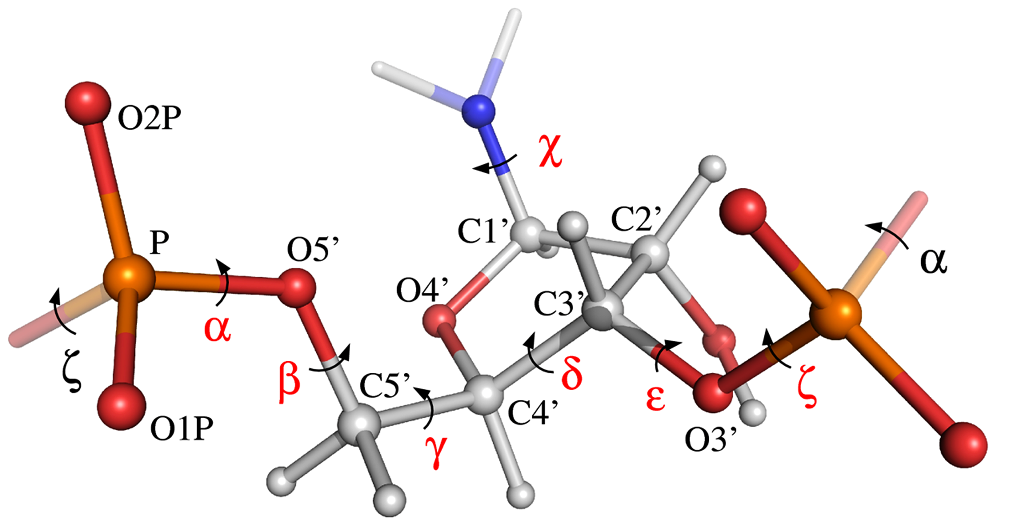
\includegraphics[width=\textwidth]{../img/str_reprezentace_uhly}
\caption{Reprezentácia RNA fragmentu pomocou siedmych uhlov. \cite{Frellsen09} }
\label{obr02:reptesentation}
\end{figure}


\indent Nástroj FARFAR \cite{Das10}, ktorý používame v našej predikcii, patrí tiež medzi knowledge based modelovacie metódy.


\section{Alignment sekvencií}
Zarovnanie dvoch sekvencií slúži na získanie informácie o tom, či sú dané sekvencie nejako evolučne, štrukturálne, alebo funkčne príbuzné. Existuje viacero druhov algoritmov zarovnania - napríklad jednoduchý dot plot vhodný na jednoduchú vizualizáciu zarovnania, heuristické metódy ako FASTA a BLAST určené na čo najrýchlejšie porovnanie sekvencie s rozsiahlou databázou ďalších sekvencií, alebo metódy počítajúce najlepšie zarovnanie určené skórovacím systémom za pomoci dynamického programovania.


\indent  V tejto práci budeme využívať semiglobálne zarovnanie pomocou algoritmu Needleman–Wunsch \cite{Needleman70}  implementovaného v programe EMBOSS \cite{Emboss}. Ako vstup algoritmus dostáva dve sekvencie dĺžiek m a n, ktoré chceme zarovnať, a hodnoty parametrov gap open (penalizácia v skóre za otvorenie medzery v zarovnaní) a gap extend (penalizácia v skóre za predĺženie medzery v zarovnaní). Algoritmus následne za pomoci dynamického programovania \ref{obr03:aln} vypočíta zarovnanie s najnižším skóre v čase aj priestore O(nm).  Výstupom algoritmu sú zarovnané sekvencie a skóre zarovnania. V zarovnaní na určitej pozícii môžu nastať tri prípady, a to zarovnanie dvoch rovnakých reziduí (match), zarovnanie dvoch odlišných reziduí (mismatch), a nakoniec zarovnanie rezidua na medzeru (gap) vloženú do druhej sekvencie. Nami používaná implementácia algoritmu nepenalizuje za medzery v zarovnaní nachádzajúce sa na začiatku alebo na konci zarovnania, preto je možné ňou zmysluplne zarovnať krátku štruktúru na časť oveľa dlhšej štruktúry.

\begin{figure}%[p]\centering
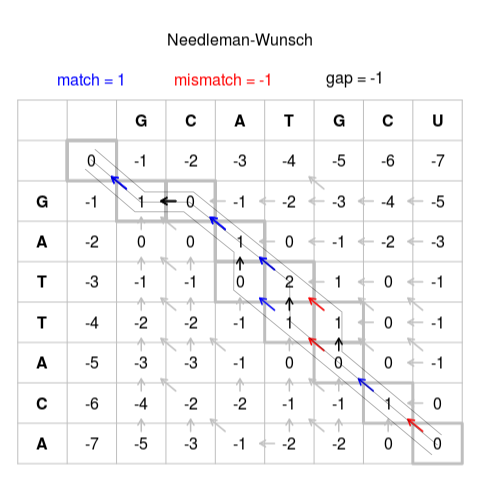
\includegraphics[width=\textwidth]{../img/needlemanwunsch}
\caption{Needleman–Wunsch algorithm (2014) Wikipedia dostupné na \url{https://en.wikipedia.org/wiki/Needleman–Wunsch\_algorithm} 27.05.2019. Príklad jedného z troch najlepších zarovnaní dvoch sekvencií: \newline GCATG-CU \newline G-ATTACA}
\label{obr03:aln}
\end{figure}


\indent Okrem globálneho poznáme aj presné lokálne zarovnanie vyriešené algoritmom Smith–Waterman \cite{Smith81}. Tento algoritmu pracuje taktiež na princípe dynamického programovania a vyhľadáva zarovnanie dvoch subsekvencií s najlepím skóre. Používa sa na nájdenie podobných regiónoch medzi dvomi sekvenciami.


\section{Homológne modelovanie}
Tvrdenie zo začiatku kapitoly, ktoré hovorí, že štruktúra si zachováva podobný tvar aj napriek tomu, že jej sekvencia postupne mutuje, umožňuje zmysluplne predikovať štruktúru na základe vzoru.  


\indent Homológne  modelovanie používa na modelovanie neznámej štruktúry zo sekvencie ešte jednu vzorovú sekvenciu (template), ktorej štruktúra je známa, teda získaná za pomoci nejakej experimentálnej metódy. Predikovanú štruktúru zvykneme nazývať cieľ (target).


\indent Prvým krokom je teda určenie vhodnej template štruktúry, pomocou ktorej budeme predikovať target štruktúru. Druhým krokom je globálne zarovnanie oboch sekvencií a získanie konzervovaných úsekov, teda úsekov v ktorých by mali byť obe štruktúry veľmi podobné. Konzervované úseky môžu byť po nejakých úpravách prenesené do cieľovej štruktúry. Z princípu vyplýva, že čím podobnejšie sekvencie budú máť target a template štruktúry, tým viac konzervovaných úsekov bude existovať a tým jednoduchšia a presnejšia by mala predikcia byť.


\indent V treťom kroku musia byť dopredikované nekonzervované (chýbajúce úseky) cieľovej štruktúry. Existujú viacero prístupov. Jedným z nich je knižnica fragmentov, kde sa do chýbajúcej medzery v cieľovej štruktúre snažíme vhodne umiestniť fragment štruktúry z knižnice, ďalším je napríklad dopredikovanie medzery ab initio alebo de novo algoritmami.


\indent Takto hotový model sa nakoniec môže optimalizovať použitím algoritmu na minimalizovanie voľnej energie, alebo sa riešia kolízie medzi jednotlivými nukleotidami.


\indent Hlavnou výhodou homológneho modelovania je, že je možné ho použiť na dlhé štruktúry. Problémom môže byť vybrať správnu template štruktúru a dopredikovanie nekonzervovaných úsekov. \ref{obr04:porovnanie}


\begin{figure}%[p]\centering
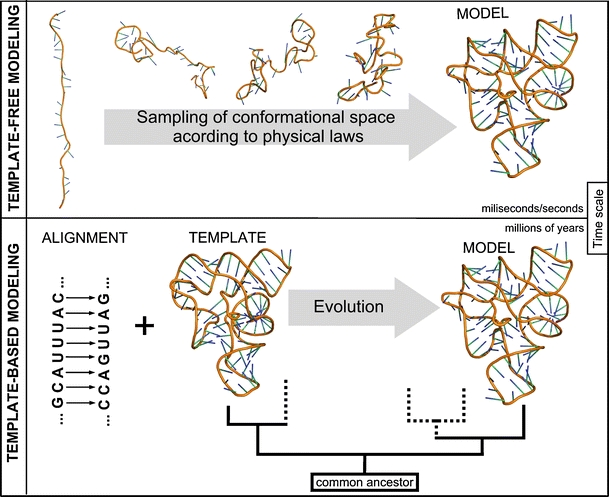
\includegraphics[width=\textwidth]{../img/template-vs-denovo}
\caption{Porovnanie princípu de novo a template based predikcie \cite{Rother11}}
\label{obr04:porovnanie}
\end{figure}


\section{Prehľad existujúcixh nástrojov}
Vďaka tomu, že počet dostupných primárnych sekvencií stále rastie rýchlejšie, ako počet experimentálne zistených terciárnych štruktúr, vzniklo mnoho nástrojov na predikciu terciárnej štruktúry RNA. \ref{tab01}


\begin{table}[b!]
\centering
\begin{tabular}{@{}lll@{}}
\toprule
Názov  & Info  & Referencia \\
\midrule
\begin{tabular}[c]{@{}l@{}}MacroMolecule\\ Builder\end{tabular} & komparatívny modeling RNA  & \cite{RNABuilder}   \\
ModeRNA & \begin{tabular}[c]{@{}l@{}}komparatívna predikcia s knižnicou \\ databázových fragmentov \\ na predikovanie medzier\end{tabular} & \cite{ModeRNA} \\
SimRNA & \begin{tabular}[c]{@{}l@{}}corase-grained model \\ s Monte Carlo samplingom štruktúr\end{tabular}    & \cite{SimRNA}  \\
FARFAR & knowledge based de novo prediktor & \cite{Das10} \\
RNAComposer & \begin{tabular}[c]{@{}l@{}}knowledge-based automatizovaná \\ predikcia štruktúry RNA \\  s využitím sekundárnej štruktúry\end{tabular} & \cite{Biesiada2016} \\
iFoldRNA & \begin{tabular}[c]{@{}l@{}}de novo predikcia RNA \\ založená na corase-grained model\end{tabular} & \cite{iFoldRNA} \\
\bottomrule

\end{tabular}

\caption{Prehľad niektorých programov určených na predikciu RNA s informáciou o type použitého algoritmu.}\label{tab01}

\end{table}


\section{ModeRNA}

ModeRNA je implementácia algoritmu komparatívneho modelovania RNA s ktorým sme porvnávali nami vyvinutý algoritmus. Je dostupná ako ModeRNA server a ponúka službu kompletnej predikcie submitovanej sekvencie (nájdenie vhodného template, zarovnanie sekvencií a vytvorenie modelu terciárnej štruktúry). Okrem toho je možné stiahnuť jej zdrojové kódy (Python) a nainštalovať a používať ju lokálne pre automatické hromadné spracovanie.


\indent Ako vstup ModeRNA požaduje zarovnanie  template a target sekvencií spolu so súradnicami jednotlivých atómov template štruktúry. Dodané zarovnanie ModeRNA nijako nemodifikuje a od jeho kvality a zvoleného template záleží výsldná presnosť predikcie. 
Zjednodušený algoritmus, ktorým ModeRNA predikuje štruktúru \cite{Rother11}: 

\begin{itemize}
\item Skopírovanie zarovnaných nukleotidov.
\item Substitúcia nukleotidov, ktoré boli zarovnané na iný nukleotid.
\item Modelovanie indelov vložením fragmentov štruktúr z knižnice obsahujúcej 131 316 fragmentov dĺžky 2-19 nukleotidov. ModeRNA najprv rýchlym filtrovaním podľa vzdialeností  prekrývajúcich sa atómov fragmentu a template-u vyberie 50 najvhodnejších kandidátov, pokúsi sa ich vložiť do medzery a pre každého kandidáta spočíta skóre, pričom vyberie jediného s najlepším skóre a  vloží ho do medzery.
\item V prípade, že predikovaná štruktúra (backbone) nie je spojitá ModeRNA sa ju pokúsi opraviť.
\end{itemize}


\section{FARFAR}

FARFAR je algoritmus de novo predikcie RNA implementovaný spolu s ďalšími bioinformatickými algoritmami a nástrojmi v balíčku Rosetta. My ho používame na predikovanie krátkych nekonzervovaných úsekov v našom algoritme.  


\indent Nástroj je shopný predikovať štruktúru iba z primárnej sekvencie. 


\indent Algoritmus pracuje tak, že nedeterministicky generuje kandidátske štruktúry z ktorých vyberie tú s najnižšou voľnou energiou. Keďže sa jedná o algoritmus typu Monte Carlo dve rôzne spustenie algoritmu môžu generovať rôzne výsledky a platí, že čím viac kandidátskych štruktúr vygenerujeme, tým zvyšujeme šancu na vygenerovanie čo najlepšej štruktúry.


\indent Z pohľadu výkonnosti platí, že čím viac nukleotidov predikujeme (včetne tých pevne daných) tým predikcia dlhšie trvá. Pre presnejšiu predstavu sme urobili porovnanie, pričom sme predikovali nekonzervovaný úsek dlhý 9 nukleotidov. Pri zahrnutí zvyšných 129 konzervovaných nukleotidov do predikcie trvalo vygenerovanie jednej štruktúry približne 13 minút. Pri totožných podmienkach a parametroch s jedinou zmenou a to, že sme do predikcie vybrali len 41 okolitých konzervovaných nukleotidov trvala predikcia jednej kandidátskej štruktúry v priemere menej ako 6 minút.


\indent Očakávaná presnosť predikcie je priamo úmerná dĺžke neznámeho predikovaného úseku. Autori algoritmu uvádzajú, že pri predikcií štruktúr dĺžky 6 až 13 nukleotidov je priemerná RMSD menšia ako 2 Å. Pri štruktúrach dlhých 13-23 nukleotidov predstavovala priemerná RMSD už 6,5 Å.


\indent Je však takisto možné dať mu na vstup pdb súbor s koordinátami niektorých nukleotidov a zakázať mu tieto nukleotidy modifikovať. 
Takisto je možné mu dodať pdb súbor s nukleotidmi a dovoliť mu, aby ho algoritmus bral ako fixovaný kus štruktúry, ktorým môže ľubovoľne  pohybovať  oproti zvyšku štruktúry.
Posledná pre nás využiteľná možnosť je dodať algoritmu sekundárnu štruktúru target molekuly. Toouto štruktúrou sa potom algoritmus pri predikcií riadi a zmenšujeje sa tak prehľadávaný priestor.

